\subsection{Introducción:}

En este ejercicio nos encargaremos del manejo de las interrupcíones del reloj, teclado y otra interrupcíon de software 0x46. Se pide:

\begin{itemize}
\item [\textit{a)}] Completar las entradas necesarias en la \textit{IDT}.
\item [\textit{b)}] Escribir la rutina asociada a la interrupcíon de reloj, de manera que por cada tick, se muestre la animacion de un cursor rotando
\item [\textit{c)}]  Escribir la rutina asociada a la interrupcíon de teclado, para aquellas teclas a utilizar en el juego, para que se imprima la misma en la pantalla
\item [\textit{d)}] Escribir la rutina asociada a la interrupcíon de software 0x46 para que modifique el valor de \textit{eax} por 0x42
\end{itemize}



\subsection{Ítem a): Completar la \textit{IDT}}

Comenzamos agregando las interrupcíones a la \textit{IDT}. Utilizamos para el reloj y el teclado las posiciones 32 y 33 respectivamente, pues son las primeras disponibles no utilizadas por el procesador. Para la interrupcíon por software, utilizamos la posicion 70, pues esta se llamara al llamar a int 0x46 $=$ 70. Las declaramos con privilegio 0, pues son de sistema y no se querria que algo externo al sistema los controle. \\
Para esto utilizamos la macro anteriormente explicada, con los siguientes parametros:

\begin{figure}[H]
\begin{center}
\minipage{0.25\textwidth}
  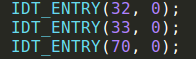
\includegraphics[width=\linewidth]{ejercicio5/idt.png}
\endminipage
\end{center}
\end{figure}

Además, las definimos en \textit{isr.h}, para luego escribir su rutina.

\begin{figure}[H]
\begin{center}
\minipage{0.25\textwidth}
  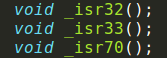
\includegraphics[width=\linewidth]{ejercicio5/isr.png}
\endminipage
\end{center}
\end{figure}

\subsection{Ítem b): Rutina del reloj}

El código es el siguiente:
\begin{figure}[H]
\begin{center}
\minipage{0.5\textwidth}
  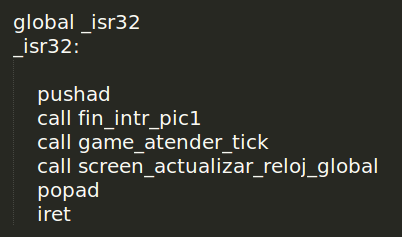
\includegraphics[width=\linewidth]{ejercicio5/rutinaReloj.png}
\endminipage
\end{center}
\end{figure}

Cada vez que se llame, la interrupcíon hara lo siguiente. Pusheara todos los registros de proposito general (lo cual en realidad no es necesario, dado que la interrupcíon no los modifica). Llamara a la fnción \textit{fin$\_$intr$\_$pic1} para decir al pic que la interrupcíon fue atendida. Luego llamara a las fnciónes \textit{game$\_$atender$\_$tick }y \textit{screen$\_$actualizar$\_$reloj$\_$global} para mostrar la animacion por pantalla. Luego popeara los registros y volvera de la interrupcíon con la instruccion iret


\subsection{Ítem c): Rutina del teclado}

El código es el siguiente:
\begin{figure}[H]
\begin{center}
\minipage{0.35\textwidth}
  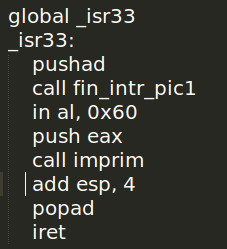
\includegraphics[width=\linewidth]{ejercicio5/rutinaTeclado.png}
\endminipage
\end{center}
\end{figure}

Igual que la interrupcíon anterior, comienza pusheando todos los registros. En este caso, es necesario preservar \textit{eax}, pues lo modificamos. Nuevamente llamamos a \textit{fin$\_$intr$\_$pic1}. Luego utilizamos la operacion \textit{in}, para mover al registro al el 
Leemos del teclado a traves del puerto 0x60 y obtenemos el scan code en \textit{eax}. Pusheamos este valor y llamamos a la función \textit{imprim} creada por nosotros. Esta fnción se encarga de traducir el scan code en una letra (en caso de que sea válido) y luego llama a la función print para mostrarlo por pantalla. Finalmente restauramos la pila, popeamos los registros y volvemos de la interrupcíon.

\subsection{Ítem d): Rutina 0x46}


El código es el siguiente:

\begin{figure}[H]
\begin{center}
\minipage{0.3\textwidth}
  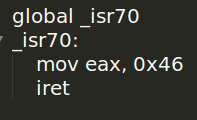
\includegraphics[width=\linewidth]{ejercicio5/rutina0x46.png}
\endminipage
\end{center}
\end{figure}

Lo único que hace esta interrupción es modificar el registro \textit{eax}. Por lo tanto no es necesario salvar los registros. Esta interrupción sera modificada mas adelante